\begin{titlepage}

\begin{center}

\huge{
Raytracing \\
Graphics Programming \\ 
Spring Semester, 2015 \\ 
\vspace*{8mm} }
\large{
IT-University of Copenhagen \\
Spring term 2015
}
\end{center}
\vspace*{7mm}

\begin{figure}[h!]
	\centering
	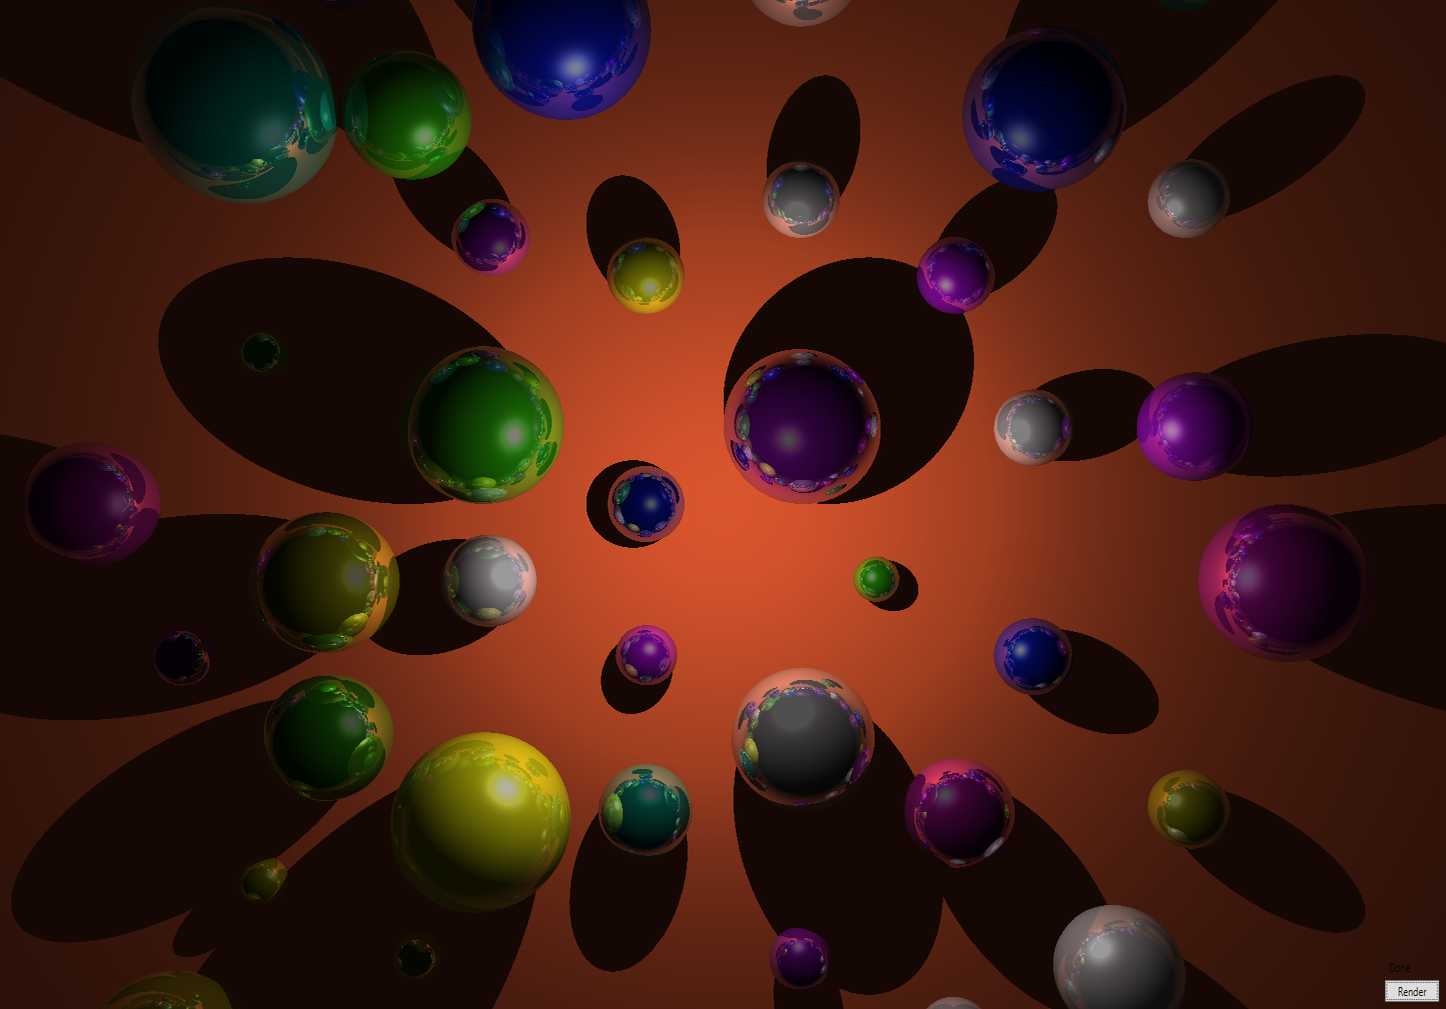
\includegraphics[width=1.0\linewidth]{Figures/GrandFinale.png}
	\caption{Screenshot from rendering produced by the delivered software}
\end{figure}



\vspace*{6mm}

\begin{center}
\begin{Large}
\textbf{Authors:} \\
\vspace*{2mm}
Anders Wind Steffensen (awia) \\
Morten Albertsen (moalb) \\ 
Rasmus Dyhr Larsen (rady)
\end{Large}
\end{center}
\vspace{3mm}
\begin{center}
\large
\textbf{Github-repository:} \\
\href{https://github.itu.dk/moalb/Graphics-Programming}{https://github.itu.dk/moalb/Graphics-Programming} \\
\normalsize 
(requires a Github.itu.dk account)
\end{center}

\end{titlepage}
\newpage